\documentclass{article}
\usepackage{graphicx}
\usepackage[margin=1.5cm]{geometry}
\usepackage{amsmath}

\begin{document}

\title{Wednesday Reading Assessment: Unit 2, Resistance and Ohm's Law}
\author{Prof. Jordan C. Hanson}

\maketitle

\section{Memory Bank}

\begin{itemize}
\item $I = \frac{dQ}{dt}$ ... Definition of current.
\item $\Delta V = I R_{\rm tot}$ ... Ohm's Law (one version).
\end{itemize}

\section{Current}

\begin{enumerate}
\item Consider Fig. \ref{fig:current1}.  (a) Indicate on the graph where the current is maximal, and indicate on the graph where the current is approaching a constant.  (b) If $\tau = 3$ ms, and $Q_{\rm M}$ = 1 nC, compute the average current.
\begin{figure}[ht]
\centering
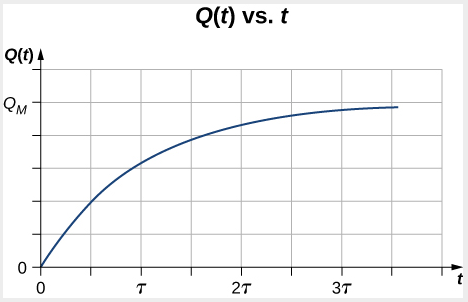
\includegraphics[width=0.35\textwidth]{current1.png}
\caption{\label{fig:current1} A graph of charge passing through a certain circuit versus time.}
\end{figure}
\end{enumerate}

\section{Ohm's Law}

\begin{enumerate}
\item Suppose a student collects the data shown in Fig. \ref{fig:ohm1}.  Deduce the total resistance in the circuit.
\begin{figure}[ht]
\centering
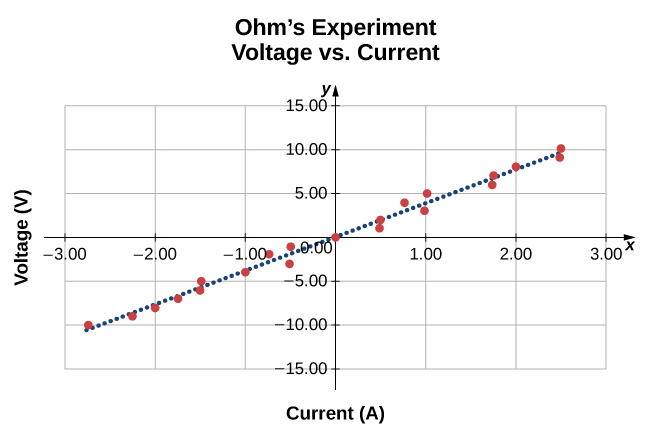
\includegraphics[width=0.5\textwidth]{ohm1.png}
\caption{\label{fig:ohm1} A graph of voltage across a circuit, versus current drawn by the circuit.}
\end{figure}
\end{enumerate}

\end{document}
